\documentclass{minimal}
\usepackage[spanish]{babel}
\usepackage{graphicx}
\usepackage[utf8]{inputenc}
\usepackage{fancyhdr}
\usepackage{lastpage}

\pagestyle{fancy}
\fancyhf{}
\rfoot{Page \thepage\hspace{1pt} de~\pageref{LastPage}}

\title{Practica 6}
\author{Guillermo Lopez Garcia}
\begin{document}
\maketitle

\textbf{Ejercicio 3.} \\
- Respecto al Speed Up con una gran numero de elementos, vemos que dividiendo el problema en un numero de hebras igual
a la cantidad hilos logicos que posee la CPU, se alcanza el Speed Up optimo.
\\
A continuación, expongo la grafica generada con gnuplot para mostrar comparación entre 
Speed Up y Numero de Hebras.
\\
\begin{figure}
  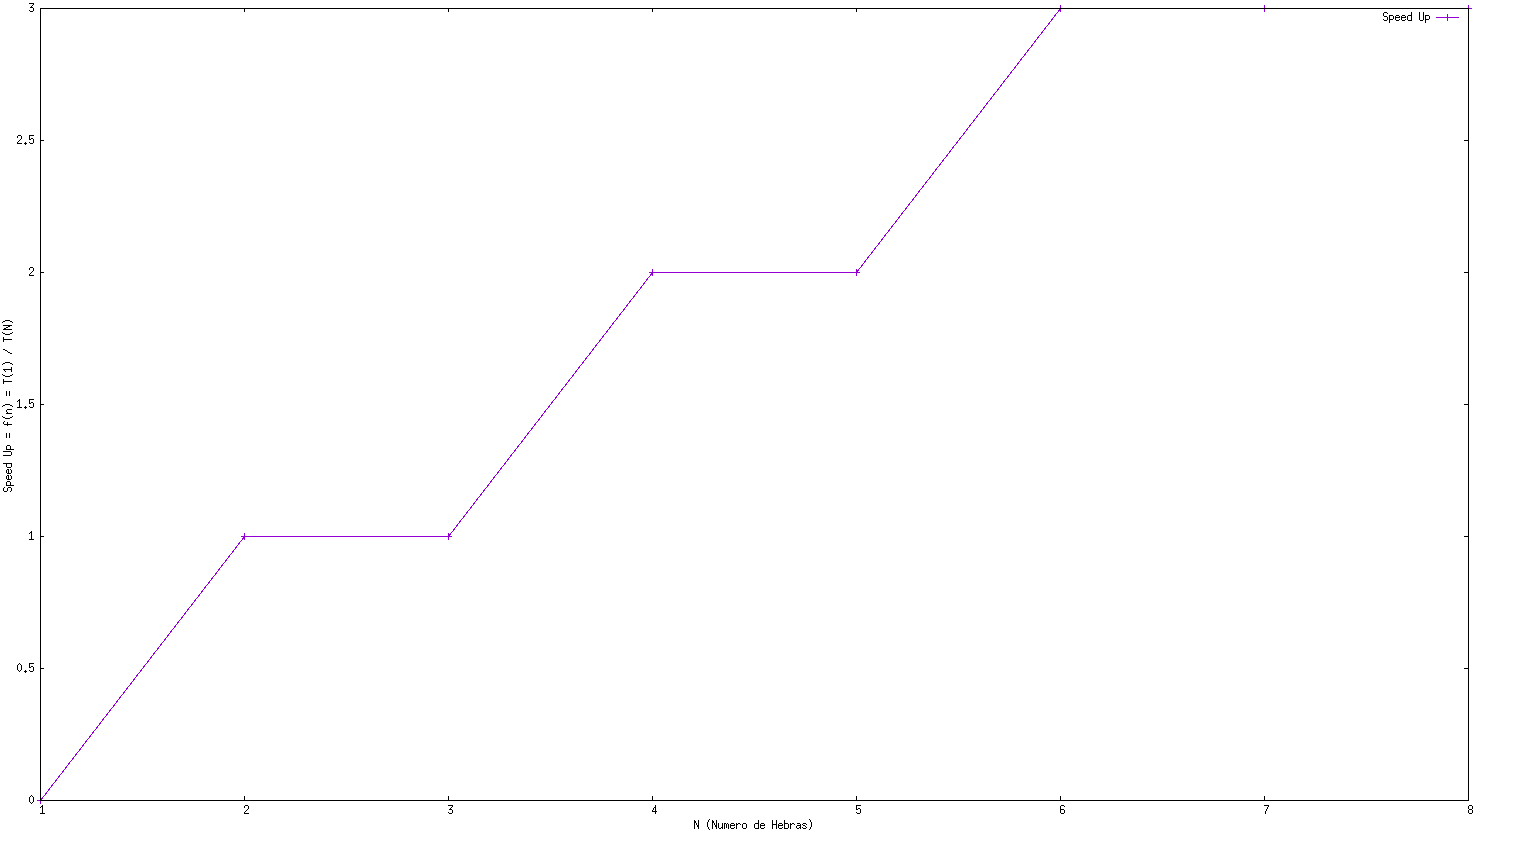
\includegraphics[width=\linewidth]{img.png}
  \caption{Comparativa de Speed Up y Nº Hebras.}
\label{fig:comp}
\end{figure}
\\
\\
Por último solo he podido probar el funcionamiento en un sistema Linux. No tuve acceso al sistema privativo y de licencia pagada Windows.

\end{document}
